\chapter{Adopting Agile Methodologies}
\label{ch:agile-solutions}

Djøf Trade Union addressed their development challenges by adopting Scrum practices that introduced structure, transparency, and empirical process control. The Scrum framework emphasizes empiricism through transparency, inspection, and adaptation \textit{\parencite{schwaber2020scrum}}. Research demonstrates that successful Agile adoption requires teams to adapt frameworks to their organizational realities \textit{\parencite{verwijs2021scrum}}. This chapter examines how they implemented Scrum practices to establish predictability and deliver value more consistently.

\section{Establishing Product Backlog Refinement}
\label{sec:refinement-process}

The introduction of structured refinement sessions fundamentally changed how work flowed into the development team. Before refinement became routine, tasks arrived ad-hoc without proper analysis of feasibility or business value. The refinement process gave the team a mechanism to break down large initiatives systematically and identify issues before developers invested time. Product Backlog refinement is an ongoing activity where the team adds detail, estimates, and order to backlog items \textit{\parencite{schwaber2020scrum}}.

Ahmed described how refinement works: before starting any project, the team runs refinement sessions where they break down epics into user stories \textbf{(Transcript: 00:05:30--00:06:00)}. The team takes business needs from stakeholders and decomposes them into manageable tasks. This allows them to deliver features incrementally. When the business side has done their preparation well and the team conducts thorough refinement where each user story has a clear purpose, projects tend to succeed \textbf{(Transcript: 00:06:00--00:06:24)}.

This practice directly addressed the legacy system problem Ahmed encountered earlier. The checkbox task that consumed weeks should never have reached the development team without first verifying legal approval and vendor accommodation. Refinement created a gate-keeping process that prevented such situations. They now question assumptions, identify dependencies, and validate feasibility during refinement rather than discovering blockers mid-implementation. The refinement process also improved transparency for stakeholders. When epics broke down into twenty user stories, stakeholders gained realistic insight into the complexity involved.

\begin{figure}[h]
\centering
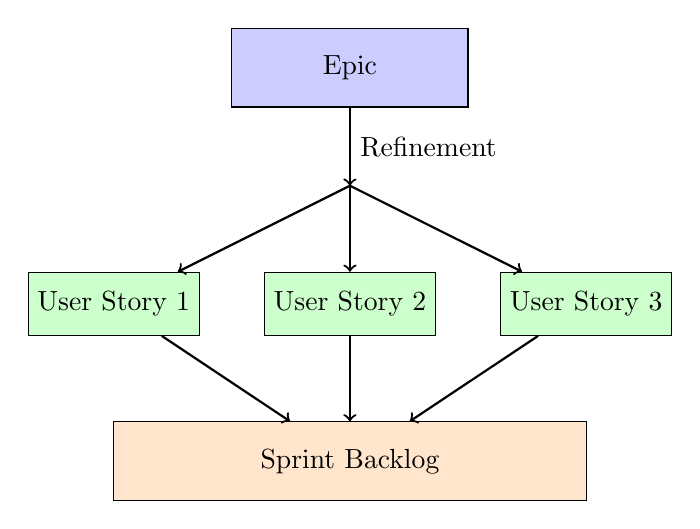
\begin{tikzpicture}
    % Epic box
    \node[draw, rectangle, fill=blue!20, minimum width=3cm, minimum height=1cm] (epic) at (0,0) {Epic};

    % Arrow down
    \draw[->, thick] (epic) -- (0,-1.5) node[midway, right] {Refinement};

    % User stories
    \node[draw, rectangle, fill=green!20, minimum width=2cm, minimum height=0.8cm] (us1) at (-3,-3) {User Story 1};
    \node[draw, rectangle, fill=green!20, minimum width=2cm, minimum height=0.8cm] (us2) at (0,-3) {User Story 2};
    \node[draw, rectangle, fill=green!20, minimum width=2cm, minimum height=0.8cm] (us3) at (3,-3) {User Story 3};

    % Arrows to user stories
    \draw[->, thick] (0,-1.5) -- (us1);
    \draw[->, thick] (0,-1.5) -- (us2);
    \draw[->, thick] (0,-1.5) -- (us3);

    % Sprint backlog
    \node[draw, rectangle, fill=orange!20, minimum width=6cm, minimum height=1cm] (backlog) at (0,-5) {Sprint Backlog};

    % Arrows to backlog
    \draw[->, thick] (us1) -- (backlog);
    \draw[->, thick] (us2) -- (backlog);
    \draw[->, thick] (us3) -- (backlog);

\end{tikzpicture}
\caption{Product Backlog Refinement Process: epics are decomposed into manageable user stories through collaborative refinement sessions.}
\label{fig:refinement-workflow}
\end{figure}


\section{Introducing Scrum Roles and Sprint Structure}
\label{sec:scrum-roles-sprints}

The adoption of defined Scrum roles brought accountability and clarity. Scrum defines three accountabilities: Product Owner, Scrum Master, and Developers, each with specific responsibilities for delivering value \textit{\parencite{schwaber2020scrum}}. The Product Owner became responsible for prioritizing the backlog in collaboration with the business, evaluating which work delivers the most value while considering technical dependencies \textbf{(Transcript: 00:14:52--00:15:22)}. This resolved the previous situation where everything seemed equally urgent. The Scrum Master role focused on maintaining the process and removing obstacles \textbf{(Transcript: 00:16:52--00:17:22)}.

Djøf Trade Union adopted two-week sprints after experimenting with different lengths. Three-week sprints proved too long, while one-week sprints were too short to deliver meaningful increments \textbf{(Transcript: 00:14:07--00:14:37)}. The two-week cadence provided sufficient time to complete user stories while maintaining rapid feedback cycles.

The team adapted Scrum pragmatically. They dropped story points because the concept proved difficult to communicate consistently \textit{\parencite{russo2021agile}}. Scrum Masters experimented with alternative estimation approaches to move away from estimates that stakeholders mistakenly interpreted as time commitments \textbf{(Transcript: 00:08:58--00:09:27)}. The team also occasionally skipped retrospectives when a sprint lacked meaningful progress to reflect on \textbf{(Transcript: 00:09:59--00:10:22)}, demonstrating their practical approach.

Sprint reviews after each sprint gave the team regular checkpoints to evaluate whether they succeeded and learn from failures \textbf{(Transcript: 00:06:48--00:07:31)}. Retrospectives provided space to refine how the team worked together. These ceremonies established inspection and adaptation cycles that were completely absent previously.

\section{Building Collaboration and Transparency}
\label{sec:collaboration-transparency}

Scrum practices fundamentally improved transparency. The visible backlog allowed stakeholders to see what the team was working on and understand capacity constraints. When stakeholders wanted new features, they could observe how those requests fit into existing priorities rather than assuming development resources were unlimited.

The sprint structure created predictability. Stakeholders knew when to expect completed features. The flexibility Ahmed mentioned as the best aspect of their approach stems from having a structured process that can accommodate change \textbf{(Transcript: 00:15:37--00:15:52)}. When business priorities shift, the team can adjust in the next sprint planning session.

Code review processes and the Azure DevOps pipeline with automated testing provided technical safeguards \textbf{(Transcript: 00:12:52--00:13:22)}. Automated tests run before code can merge. A colleague must review and approve the code before it progresses. The deployment pipeline moves code through development, test, and production environments systematically, creating quality gates at each stage. Delivering a Done increment every Sprint reduces the risk of undone work accumulating and disrupting future development \textit{\parencite{liberators_scrum}}.

Collaboration within the team also improved. Developers could focus on defined sprint goals rather than constantly reacting to incoming requests. The Product Owner acted as a buffer, managing stakeholder expectations and protecting the team from excessive interruptions. This allowed developers to work more proactively and build solutions with proper consideration for technical quality.

\begin{figure}[h]
\centering
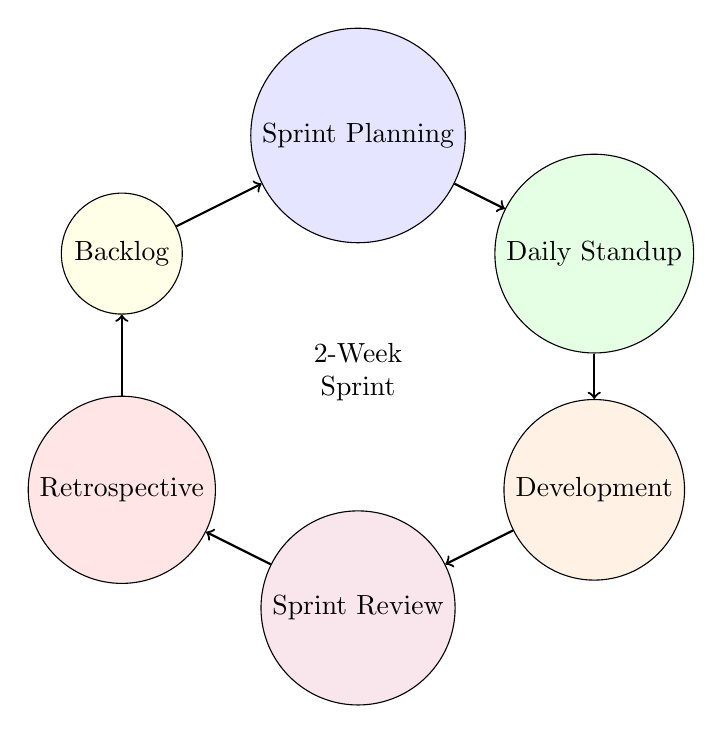
\begin{tikzpicture}
    % Sprint cycle circle
    \node[draw, circle, fill=blue!10, minimum size=1.5cm] (planning) at (0,3) {Sprint Planning};
    \node[draw, circle, fill=green!10, minimum size=1.5cm] (daily) at (3,1.5) {Daily Standup};
    \node[draw, circle, fill=orange!10, minimum size=1.5cm] (development) at (3,-1.5) {Development};
    \node[draw, circle, fill=purple!10, minimum size=1.5cm] (review) at (0,-3) {Sprint Review};
    \node[draw, circle, fill=red!10, minimum size=1.5cm] (retro) at (-3,-1.5) {Retrospective};
    \node[draw, circle, fill=yellow!10, minimum size=1.5cm] (backlog) at (-3,1.5) {Backlog};

    % Arrows showing cycle
    \draw[->, thick] (planning) -- (daily);
    \draw[->, thick] (daily) -- (development);
    \draw[->, thick] (development) -- (review);
    \draw[->, thick] (review) -- (retro);
    \draw[->, thick] (retro) -- (backlog);
    \draw[->, thick] (backlog) -- (planning);

    % Center label
    \node[align=center] at (0,0) {2-Week\\Sprint};

\end{tikzpicture}
\caption{Sprint Cycle: Ahmed's team follows a two-week sprint cadence with regular ceremonies for planning, coordination, review, and continuous improvement.}
\label{fig:sprint-cycle}
\end{figure}


\section{Addressing Change Resistance}
\label{sec:change-resistance}

Not everyone embraced Scrum immediately. Stakeholders accustomed to making direct requests to developers found the Product Owner intermediary frustrating. Developers who valued autonomy sometimes viewed ceremonies as unnecessary overhead. The organization addressed resistance through demonstrated results. When sprints consistently delivered working software, skeptics recognized the value. Leadership support proved critical. Management allocated time for Scrum ceremonies and protected teams from pressure to bypass the process during urgent situations.
